\documentclass[letterpaper,10pt]{article}
\usepackage[utf8]{inputenc}
\usepackage{amsmath}
\usepackage{amsfonts}
\usepackage{amssymb}
\usepackage{graphicx}

\newcommand{\comment}[1]{{\textbf{#1}}}
\newcommand{\cotwo}{CO$_2$ }
\newcommand{\COtwo}[1]{CO$_2$ }
\newcommand{\erf}{\text{erf}}
\newcommand{\bu}{\boldsymbol{u}}
\newcommand{\bv}{\boldsymbol{v}}
\newcommand{\bx}{\boldsymbol{x}}
\newcommand{\bz}{\hat{\boldsymbol{z}}}
\newcommand{\grad}{\boldsymbol{\nabla}}
\newcommand{\cL}{\boldsymbol{\mathcal{L}}}
\newcommand{\cA}{\boldsymbol{\mathcal{A}}}
\newcommand{\cI}{\boldsymbol{\mathcal{I}}}
\newcommand{\cW}{\boldsymbol{\mathcal{W}}}
\newcommand{\cB}{\boldsymbol{\mathcal{B}}}
\newcommand{\cR}{\boldsymbol{\mathcal{R}}}
\newcommand{\cLam}{\boldsymbol{\boldsymbol{\Lambda}}}
\newcommand{\cOmega}{\boldsymbol{\boldsymbol{\Omega}}}

\newcommand{\tc}{t_*}
\newcommand{\prt}{\boldsymbol{\xi}}
\newcommand{\nrm}{{\|\cdot\|}}
\newcommand{\norm}[1]{{\|#1\|}}
\newcommand{\obs}{o}
\newcommand{\inc}{i}

\newcommand{\mx}{{
\begin{bmatrix} 
 x \\ y
\end{bmatrix}
}}

\newcommand{\Rot}{{
\begin{bmatrix} 
  \cos \omega t & \sin \omega t \\
 -\sin \omega t & \cos \omega t
\end{bmatrix}
}}

\newcommand{\Rotinv}{{
\begin{bmatrix} 
  \cos \omega t & -\sin \omega t \\
  \sin \omega t &  \cos \omega t
\end{bmatrix}
}}

\newcommand{\Bmat}{{
\begin{bmatrix} 
 -\sigma & \gamma \\
 0  & -\sigma
\end{bmatrix}
}}

\newcommand{\Btmat}{{
\begin{bmatrix} 
 \alpha t & \gamma \\
 0  & \alpha t
\end{bmatrix}
}}


%opening
\title{Freeze your coefficients. Now.}
\author{Anja Slim and Shreyas Mandre}
\begin{document}
\maketitle

\begin{abstract}
We provide a method for determining the onset of linear instability for general transient base states, and illustrate its application to solutal convection in porous media relevant for carbon dioxide sequestration in underground aquifers. 
This method is based on the amplification of the most dangerous perturbation induced on the least amplified norm. 
We define the threshold time for the growth of at least one perturbation in {\em every} norm (the onset of instability) agrees exactly with threshold found using frozen coefficient analysis. 
We construct a sufficient condition for verifying the consistency of frozen coefficient analysis to predict this onset. 
We also derive a necessary and sufficient condition.
\end{abstract}
\section{Introduction}
Linear stability of time-dependent base states appears in many fields from atmospherics sciences, ocean sciences, thin film flows, geological sciences and engineering, and whatever else. 
A common method employed is to freeze the background flow and thus the linear operator appearing in the dynamics, and determine the stability based on the eigenvalues of this operator. 
Underlying this method is a tacit assumption that the perturbations grow or decay much faster than the base flow changes. 
This method is inconsistent for determining the onset of the instability in time, because at onset the perturbations neither grow nor decay.
Moreover, it is not clear what to use when the timescales are not separated.
Indeed, examples where the eigenvalues of frozen coefficient operator are negative but perturbations grow exponentially are well known. 
The existence of these examples, and the absence of a clear criteria for the validity of the frozen coefficient analysis jeopardizes the results obtained by freezing the coefficients.

Fear not. We will salvage the situation in this paper. (Summary of our results.)

\section{Background linear algebra}
A matrix $\cA$ induces an amplification of a norm $\nrm$ defined as
\begin{equation}
a_\nrm = \max_{\prt} \frac{\norm{\cA \prt}}{\norm{\prt}}.
\end{equation}
The least possible amplification induced on any norm is
\begin{equation}
a = \min_{\nrm} a_\nrm = \min_{\nrm} \max_{\prt} \frac{\norm{\cA \prt}}{\norm{\prt}}.
\end{equation}

The solution to this optimization problem is 
\begin{equation} \label{eq:RHO}
a(t_\obs,t_\inc) = \rho(\cA),
\end{equation}
where $\rho(\cA)$ is the spectral radius of $\cA$, the largest magnitude of the eigenvalues of $\cA$.  This results from two theorems of finite-dimensional linear algebra.
The first states that for every vector norm $\rho(\cA) \le a(t_\obs,t_\inc)$, as can be easily verified by substituting the eigenvector corresponding to the largest magnitude eigenvalue of $\cA$. 
The second states that there exists a vector norm for which the spectral radius comes arbitrarily close to $a(t_\obs,t_\inc)$ \cite{bulirsch2002introduction}; {\it i.e.} for at least one $\nrm$ and $\epsilon>0$, $\rho (\cA) + \epsilon > a(t_\obs,t_\inc)$. 
Combining the conclusions proves our claim.% that $a(t_\obs, t_\inc) = \rho(\cA)$. 
The least amplified norm is the $L_\infty$ norm in the transformed space using eigenvectors of $A$ as the basis.

\section{Salvaging frozen coefficients}
Describe how we can verify if the results from frozen coefficients are valid using the growth rate of the least amplified norm at threshold.

\section{General case}
The system may be formally integrated as
\begin{equation} \label{eq:PROP}
\prt (t_\obs) = \cA(t_\obs, t_\inc) \prt (t_\inc), 
\end{equation}
where $\cA (t_\obs, t_\inc)$ is the propagator for the linear system, a linear operator transforming an initial condition at time $t_\inc$ into a solution of the initial value problem at time $t_\obs$.  
The propagator satiesfies $d\cA/dt = \cL \cA$ with initial condition $\cA=\cI$ at $t=t_\inc$.  
The amplification $a(t_\obs, t_\inc)$ of the most dangerous perturbation on the least amplified norm is 
\begin{equation}
a(t_\obs, t_\inc) = \rho(\cA(t_\obs, t_\inc)).
\end{equation}

\bibliography{timevariant,others}
\bibliographystyle{plain}

\newpage
\section*{Supplementary Information}
\setcounter{page}{1}
Here we consider the mechanism for the transience of the linear operator to induce growth even if the frozen coefficient matrix has eigenvalues with negative real parts. 
Many examples of such behavior exist in the literature, but no clear criteria is identified for its occurrence. 

\subsection*{Constant eigenvectors}
If the eigenvectors of $\cL(t)$ do not vary with time, then frozen coefficient analysis is correct. Note that in this case $\cL(t_1)$ commutes with $\cL(t_2)$ for any $t_1$, $t_2$.

\textbf{Justification}: If $\cL$ has the same set of eigenvectors for all $t$, then $\cL$ may be written in terms of its Jordan normal form $\Lambda$ and the matrix of eigenvectors as columns $\cW$ as $\cL = \cW \cLam(t) \cW^{-1}$. Transforming $\bu = \cW \bv$ yields 
\begin{equation}
 \frac{d\bv}{dt} = \cLam(t) \bv.
\end{equation}
The solution for $\bv$ is 
\begin{equation}
\bv = \exp \left[ \int_{t_1}^t \cLam(s)~ds \right] \bv(t=t_1),
\end{equation}
and for $\bu$ is
\begin{equation}
\bu = \cW \exp \left[ \int_{t_1}^t \cLam(s)~ds \right] \cW^{-1} \bu(t=t_1).
\end{equation}
Thus the amplification induced is the integral of the instantaneous growth (as determined from frozen coefficient analysis) along the characteristic directions of $\cL$. This analysis also shows that for the transient results to differ from frozen coefficient analysis it is necessary for the eigenvectors to change with time.

\subsection*{Orthogonal eigenvectors}
If the eigenvectors are orthogonal, frozen coefficient analysis gives the correct result. For this case, $\cL(t)$ is symmetric (or self-adjoint).

Let us denote the diagonalization of $\cL$ as $\cL(t) = \cW(t) \cLam(t) \cW(t)^T$, where $\cW(t)$ is the matrix composed of eigenvectors as columns, and $\cLam(t)$ is the diagonal matrix of eigenvalues. Because the eigenvectors are orthonormal at every time, the rate of change of $\cW$ can be described using a skew-symmetric rotation matrix $\cOmega$ as $d \cW/dt = \cW \cOmega$. Transforming $u = \cW v$ yields
\begin{equation}
 \frac{d\bv}{dt} = (\cLam - \cOmega) \bv.
\end{equation}
Take dot product of this equation with $\bv^T$ yields
\begin{equation}
\frac{d}{dt} \bv^T \bv = \bv^T \cLam \bv. 
\end{equation}
Expanding the right hand side of this equation component-wise shows that if each of diagonal elements of $\cLam$ (the eigenvalues of $\cL$) is negative, the right hand side is also negative.

\subsection*{Time varying non-orthogonal eigenvectors: example one}
If the eigenvectors are not orthogonal, and are varying with time, frozen coefficient can yield unreliable results as the following example demonstrates. Consider the combination of linear system with shearing rate $\cB$, but the direction of shear rotating constantly according to a matrix $\cR$.
\begin{equation}
 \frac{d\bu}{dt} = \cR \cB \cR^{-1} \bu, \text{ where } \cB = \Bmat, \text{ and } \cR(\omega t) = \Rot.
\end{equation}
The frozen coefficient eigenvalues of $\cR \cB \cR^{-1}$ are the same as the eigenvalues of $\cB$, which are $-\sigma$ (we consider $\sigma>0$, so the eigenvalues are negative). 
By itself, the matrix $\cB$ rotates the state vector in the clock-wise direction at the rate $\gamma/2$ and stretches it at the rate $-\sigma \pm \gamma/2$ along the $[1, 1]$ and $[1, -1]$ directions respectively. 
The rotation matrix $\cR$ further continuously rotates the direction of shear clockwise at a rate $\omega$; it satisfies
\begin{equation}
 \frac{d\cR}{dt} = \omega \begin{bmatrix} 0 & -1 \\ 1 & 0 \end{bmatrix} \cR = \cOmega \cR.
\end{equation}

To demonstrate that this system can exhibit growth, transform $\bu = \cR \bv$ to yield an autonomous system
\begin{equation}
 \frac{d\bv}{dt} = (\cB - \cOmega) \bv, \quad \cB - \cOmega = \begin{bmatrix} -\sigma & \gamma-\omega \\ \omega & -\sigma \end{bmatrix}.
\end{equation} 
          
The matrix $\cB - \cOmega$ has eigenvalues $\mu = -\sigma \pm \sqrt{\gamma \omega -\omega^2}$. The maximum possible value for the term in the square-root is $\gamma^2/4$ when $\omega = \gamma/2$. Thus $\mu$ has a positive real part if $\sigma < \gamma/2$. (For example, if $\gamma = 1$, $\omega = 1/2$ and $\sigma < 1/2$, then the real part of $\mu$ is positive.)  

In other words, if the direction of shear rotates constantly to compensate for the rotation of the state vector it induces ($\omega = \gamma/2$), and the isotropic contraction rate is overcome by the stretching due to shear ($\sigma<\gamma/2$), the state vector can sustain the growth. Such stretching due to shear is also present if the rotation were absent, but the rate of stretching is only sustained because of the rotation aligning the rate of stretching with the state vector. 

This examples illustrates how the rotation rate of the reference frame is a critical parameter in determining if eigenvalues of the linear operator with frozen coefficient yields results consistent with the our intuitive notion of stability.

\subsection*{Time varying non-orthogonal eigenvectors: example two}
This example demonstrates the possibility that the onset of instability may not be detected by frozen coefficient analysis.

Consider 
\begin{equation}
 \frac{d\bu}{dt} = \cR \cB \cR^{-1} \bu, \text{ where } \cB = \Btmat, \text{ and } \cR \text { as before.}
\end{equation}
The eigenvalues of the frozen coefficient matrix $\cR \cB \cR^{-1}$ are $\alpha t$, and onset of instability occurs at $t=0$ (we assume $\alpha>0$). Transforming to a rotating frame using $\bu = \cR \bv$ yields
\begin{equation}
 \frac{d\bv}{dt} = (\cB - \cOmega) \bv, \quad \cB - \cOmega = \begin{bmatrix} \alpha t & \gamma-\omega \\ \omega & \alpha t \end{bmatrix}.
\end{equation}
Freezing $(\cB - \cOmega)$ yields eigenvalues $\alpha t \pm \sigma$, where $\sigma = \sqrt{\omega (\gamma-\omega)}$ (we assume $\omega$ and $\gamma$ are such that $\sigma$ is real). Setting the eigenvalue with the largest real part to zero yields $t_c = -\sigma/\alpha$, which differs from the result obtained by freezing $\cR \cB \cR^{-1}$. 

A closed form solution for this system is $\bv(t) = \cA(t,t_0) \bv(t_0)$, where
\begin{equation}
 \cA(t,t_0) = \exp \left(\dfrac{\alpha t^2}{2} - \dfrac{\alpha t_0^2}{2} \right)
 \begin{bmatrix}
                                 \cosh \sigma (t-t_0) & \dfrac{\sigma}{\omega} \sinh \sigma(t-t_0) \\
 \dfrac{\sigma}{(\gamma-\omega)} \sinh \sigma (t-t_0) &                         \cosh\sigma (t-t_0)
 \end{bmatrix}
.
\end{equation}
The propagator for $\bu$ can also be written to be $\bu(t) = \cR(\omega t) \cA(t, t_0) \cR(\omega t_0)$, which has eigenvalues different from $\cA$. 
Furthermore, the propagator for the solution $\bw = \cR(\omega_0 t) \bu$ in a frame rotating at the rate $\omega_0$ is $\tilde{\cA}(t,t_0) = \cR((\omega+\omega_0)t) \cA(t, t_0) \cR((\omega+\omega_0)t_0)\cR$.
The spectral radius of $\cA$ is
\begin{equation}
 \rho(\cA (t, t_0)) = \exp \left[ \dfrac{\alpha t^2}{2} - \dfrac{\alpha t_0^2}{2} + \sigma (t_0-t) \right]. 
\end{equation}
This spectral radius is greater than unity if $\dfrac{\alpha t^2}{2} - \dfrac{\alpha t_0^2}{2} + \sigma (t_0-t)>0$ for the smallest $t>t_0$. 
This condition first occurs for $t_0 = -\sigma/\alpha$, and $t=t_0^{+}$. 
Depending on the relative sizes and signs of $\sigma$ and $\alpha$, the onset can happen at an arbitrary time before or after the prediction made from naively freezing the coefficients of $\cB$.

\begin{figure}
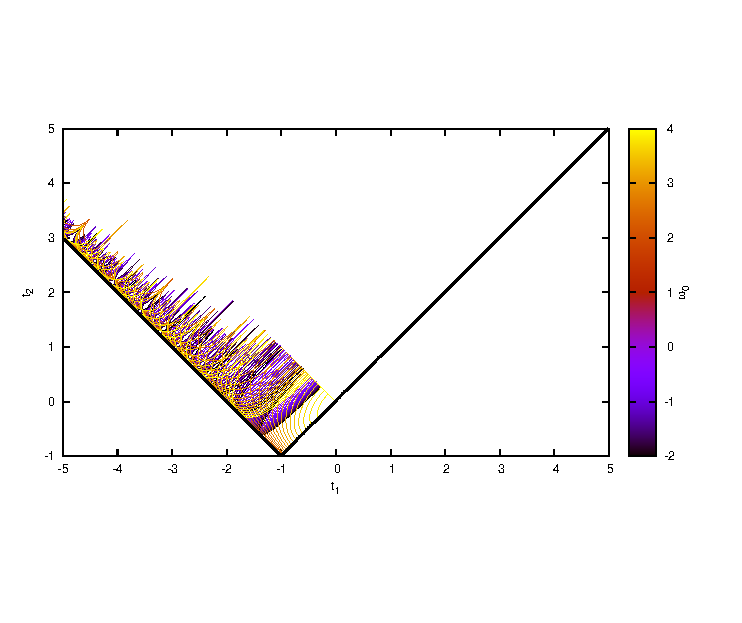
\includegraphics{Figures/beta1/beta}
\caption{Neutral curves for the spectral radius of the propagator in a frame rotating with rate $\omega_0$ for example two with $\alpha=2$, $\gamma=4$, $\omega=2$. The earliest onset of growth appears at $t_1=t_2=-\gamma/2\alpha=-1$. The envelope of these neutral curves corresponds to the neutral curve for $\omega_0 = \omega = 2$. }
\end{figure}


While these examples employ a degerate matrix $\cB$ to demonstrate the effect of a time-varying linear operator, the underlying qualitative explanation is generally applicable. For a non-degenerate case, see the example by Knboloch and Merryfield (19??).
\end{document}
